\documentclass[onlytextwidth, aspectratio=169]{beamer}
\usepackage[utf8]{inputenc}
\usepackage{microtype}
\usepackage{amsmath}
\usepackage{amssymb}
\usepackage[nomessages]{fp} %\FPeval{\var-name}{2*sin(pi/6)}
\usepackage{siunitx} %units in math. eg 20\milli\meter
\usepackage{yhmath} % for arcs, overparenth command
\usepackage{tikz} %graphics
\usetikzlibrary{quotes, angles, arrows, arrows.meta}
%\usepackage{graphicx} already loaded by beamer class
%consider setting \graphicspath{{images/}}
%\parskip ?? to avoid paragraph indent
\usepackage{multicol} %may not need this package, just columns environment
\usepackage{venndiagram}

\subtitle[BECA]{Bronx Early College Academy}
\author[Huson]{Christopher J. Huson PhD}

\setbeamertemplate{headline}{\vskip2mm 
  \, BECA / \insertshortauthor \, / \inserttitle
  \hfill 
  \insertsection
  }

%Tick mark commands
\newcommand\ticks{}
  \def\ticks{{Bar[scale=2]}-{Bar[scale=2]}}
\newcommand\paraticks{}
  \def\paraticks{{Straight Barb[reversed, scale=2]}-{Straight Barb[scale=2]}}

\title{Geometry Unit 6: Analytic Geometry}
\date{7 December 2022 - 13 January 2023}

\begin{document}
\frame{\titlepage}
\section[Outline]{}
\frame{\tableofcontents}

\section{6.1 Midpoint formula \hfill 8 December \,}
\begin{frame}{Learning Target: I can plot a midpoint on the plane}
  {HSG.CO.C.9 Prove theorems about lines and angles  \hfill \alert{6.1 Thursday 8 December}}
  \begin{block}{Do Now}
    \begin{enumerate}
      \item Review your Jumprope grades
      \item Find the midpoint $M$ of $\overline{AB}$
    \end{enumerate}
    \begin{center}
      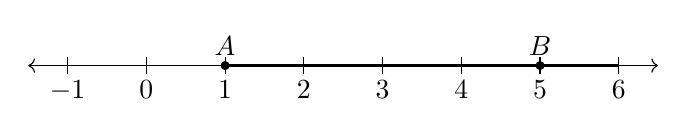
\begin{tikzpicture}
        \draw[<->] (-1.5,0)--(6.5,0);
        \foreach \x in {-1,...,6}
          \draw[shift={(\x,0)}] (0pt,-3pt)--(0pt,3pt) node[below=5pt]{$\x$};
        \draw[fill] (1,0) circle [radius=0.05] node[above]{$A$};
        \draw[fill] (5,0) circle [radius=0.05] node[above]{$B$};
        \draw[thick] (1,0)--(6,0);
      \end{tikzpicture}
    \end{center} 
  \end{block}
    Lesson: Midpoint and average, classwork practice \\
    Homework: Deltamath midpoint practice (optional extension)
\end{frame}

\begin{frame}{What do you know about the coordinate plane?}
    \begin{columns}
      \column{0.7\textwidth}
      \begin{description}
        \item[Coordinates] Values locating a point on a plane $(x,y)$
        \item[Axis] The two number lines, $x$ and $y$-axis
        \item[Origin] The center of the plane, $(0,0)$
        \item[Quadrant] The four quarters of the plane 
      \end{description}
      \column{0.3\textwidth}
      \begin{flushright}
        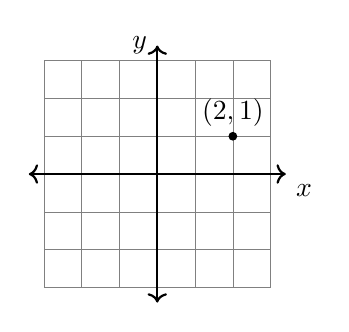
\begin{tikzpicture}[scale=.48]
          \draw [help lines] (-3,-3) grid (3,3);
          \draw [thick, <->] (-3.4,0) -- (3.4,0) node [below right] {$x$};
          \draw [thick, <->] (0,-3.4)--(0,3.4) node [left] {$y$};
          \draw [fill] (2,1) circle [radius=0.1] node[above] {$(2,1)$};
        \end{tikzpicture}
      \end{flushright}
    \end{columns} \vspace{0.5cm}
  \end{frame}


\begin{frame}{The midpoint formula}
  \begin{columns}
    \column{0.5\textwidth}
    Given $A(x_A,y_A)$, $B(x_B,y_B)$, midpoint $$\displaystyle M = \left(\frac{x_A+x_B}{2}, \frac{y_A+y_B}{2}\right)$$ \vspace{0.5cm}
    \column{0.5\textwidth}
    \begin{flushright}
      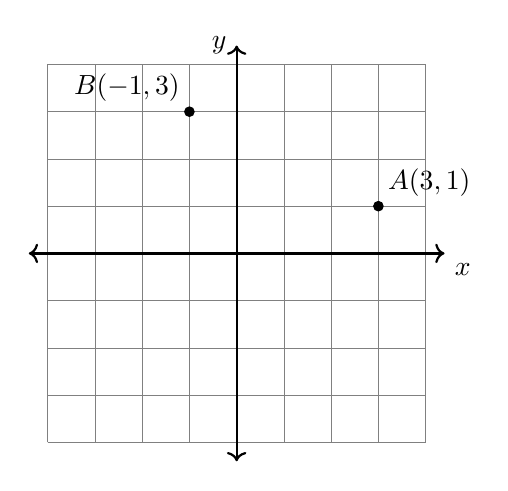
\begin{tikzpicture}[scale=0.6]
        \draw [help lines] (-4,-4) grid (4,4);
        \draw [thick, <->] (-4.4,0) -- (4.4,0) node [below right] {$x$};
        \draw [thick, <->] (0,-4.4)--(0,4.4) node [left] {$y$};
        \draw [fill] (3,1) circle [radius=0.1] node[above right] {$A(3,1)$};
        \draw [fill] (-1,3) circle [radius=0.1] node[above left] {$B(-1,3)$};
      \end{tikzpicture}
    \end{flushright}
  \end{columns} \vspace{0.5cm}
\end{frame}

\section{6.2 Slope-intercept form \hfill 9 December \,}
\begin{frame}{Learning Target: I can use slope-intercept form of linear equations}
  {HSG.CO.C.9 Prove theorems about lines and angles  \hfill \alert{6.2 Friday 9 December}}
  \begin{columns}
    \column{0.5\textwidth}
      Do Now: Find the midpoint $M$ of $\overline{AB}$ \\[1cm]
      Lesson: Slope, $y$-intercept, linear equations \\
      Homework: Deltamath graphing practice (optional extension)
    \column{0.5\textwidth}
    \begin{flushright}
      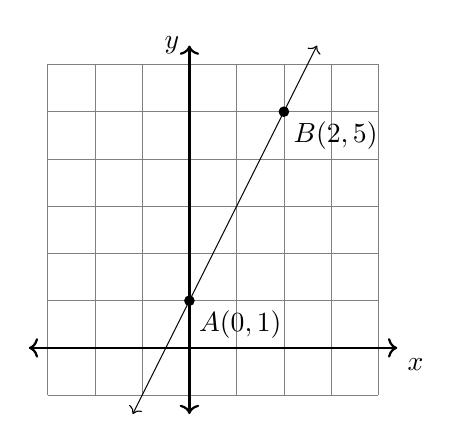
\begin{tikzpicture}[scale=0.6]
        \draw[help lines] (-3,-1) grid (4,6);
        \draw[thick, <->] (-3.4,0) -- (4.4,0) node [below right] {$x$};
        \draw[thick, <->] (0,-1.4)--(0,6.4) node [left] {$y$};
        \draw[<->,domain=-1.2:2.7] plot (\x, 2*\x+1) ;
        \draw [fill] (0,1) circle [radius=0.1] node[below right] {$A(0,1)$};
        \draw [fill] (2,5) circle [radius=0.1] node[below right] {$B(2,5)$};
      \end{tikzpicture}
    \end{flushright}
  \end{columns}
\end{frame}

\begin{frame}{Linear equations of the form $y=mx+b$}
  \begin{columns}
    \column{0.6\textwidth}
    \begin{description}
      \item[Linear] Straight, constant rate of change
      \item[Intercept] Where the line crosses the axis
      \item[$b$] $y$-intercept, point $(0,b)$ when $x=0$
      \item[Increasing] Going up. $y$ increases as $x$ increases
      \item[Decreasing] Going down. $y$ decreases as $x$ increases
      \item[$m$, slope] How steep the line is 
      $$m=\frac{rise}{run}=\frac{y_B-y_A}{x_B-x_A}$$
    \end{description}
    \column{0.4\textwidth}
    \begin{flushright}
      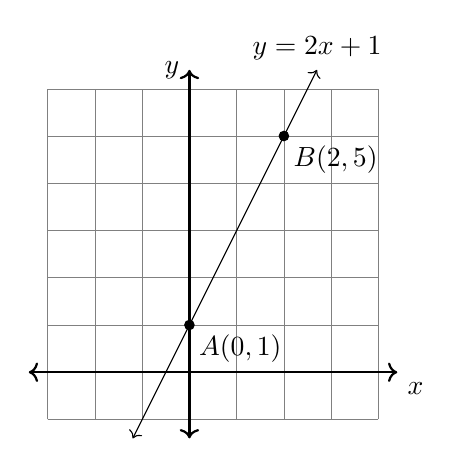
\begin{tikzpicture}[scale=0.6]
        \draw[help lines] (-3,-1) grid (4,6);
        \draw[thick, <->] (-3.4,0) -- (4.4,0) node [below right] {$x$};
        \draw[thick, <->] (0,-1.4)--(0,6.4) node [left] {$y$};
        \draw[<->,domain=-1.2:2.7] plot (\x, 2*\x+1) node[above]{$y=2x+1$};
        \draw [fill] (0,1) circle [radius=0.1] node[below right] {$A(0,1)$};
        \draw [fill] (2,5) circle [radius=0.1] node[below right] {$B(2,5)$};
      \end{tikzpicture}
    \end{flushright}
  \end{columns}
\end{frame}

\end{document}